% Options for packages loaded elsewhere
\PassOptionsToPackage{unicode}{hyperref}
\PassOptionsToPackage{hyphens}{url}
%
\documentclass[
  12pt,
]{article}
\usepackage{amsmath,amssymb}
\usepackage{lmodern}
\usepackage{iftex}
\ifPDFTeX
  \usepackage[T1]{fontenc}
  \usepackage[utf8]{inputenc}
  \usepackage{textcomp} % provide euro and other symbols
\else % if luatex or xetex
  \usepackage{unicode-math}
  \defaultfontfeatures{Scale=MatchLowercase}
  \defaultfontfeatures[\rmfamily]{Ligatures=TeX,Scale=1}
\fi
% Use upquote if available, for straight quotes in verbatim environments
\IfFileExists{upquote.sty}{\usepackage{upquote}}{}
\IfFileExists{microtype.sty}{% use microtype if available
  \usepackage[]{microtype}
  \UseMicrotypeSet[protrusion]{basicmath} % disable protrusion for tt fonts
}{}
\usepackage{xcolor}
\IfFileExists{xurl.sty}{\usepackage{xurl}}{} % add URL line breaks if available
\IfFileExists{bookmark.sty}{\usepackage{bookmark}}{\usepackage{hyperref}}
\hypersetup{
  pdftitle={Limits of Media Effects},
  pdfkeywords={Public Opinion, Media Effects, News Framing, Opinion Formation, Emphasis Framing, Conditions of Media Effects.},
  hidelinks,
  pdfcreator={LaTeX via pandoc}}
\urlstyle{same} % disable monospaced font for URLs
\usepackage[margin=1.5in]{geometry}
\usepackage{longtable,booktabs,array}
\usepackage{calc} % for calculating minipage widths
% Correct order of tables after \paragraph or \subparagraph
\usepackage{etoolbox}
\makeatletter
\patchcmd\longtable{\par}{\if@noskipsec\mbox{}\fi\par}{}{}
\makeatother
% Allow footnotes in longtable head/foot
\IfFileExists{footnotehyper.sty}{\usepackage{footnotehyper}}{\usepackage{footnote}}
\makesavenoteenv{longtable}
\usepackage{graphicx}
\makeatletter
\def\maxwidth{\ifdim\Gin@nat@width>\linewidth\linewidth\else\Gin@nat@width\fi}
\def\maxheight{\ifdim\Gin@nat@height>\textheight\textheight\else\Gin@nat@height\fi}
\makeatother
% Scale images if necessary, so that they will not overflow the page
% margins by default, and it is still possible to overwrite the defaults
% using explicit options in \includegraphics[width, height, ...]{}
\setkeys{Gin}{width=\maxwidth,height=\maxheight,keepaspectratio}
% Set default figure placement to htbp
\makeatletter
\def\fps@figure{htbp}
\makeatother
\setlength{\emergencystretch}{3em} % prevent overfull lines
\providecommand{\tightlist}{%
  \setlength{\itemsep}{0pt}\setlength{\parskip}{0pt}}
\setcounter{secnumdepth}{-\maxdimen} % remove section numbering
\newlength{\cslhangindent}
\setlength{\cslhangindent}{1.5em}
\newlength{\csllabelwidth}
\setlength{\csllabelwidth}{3em}
\newlength{\cslentryspacingunit} % times entry-spacing
\setlength{\cslentryspacingunit}{\parskip}
\newenvironment{CSLReferences}[2] % #1 hanging-ident, #2 entry spacing
 {% don't indent paragraphs
  \setlength{\parindent}{0pt}
  % turn on hanging indent if param 1 is 1
  \ifodd #1
  \let\oldpar\par
  \def\par{\hangindent=\cslhangindent\oldpar}
  \fi
  % set entry spacing
  \setlength{\parskip}{#2\cslentryspacingunit}
 }%
 {}
\usepackage{calc}
\newcommand{\CSLBlock}[1]{#1\hfill\break}
\newcommand{\CSLLeftMargin}[1]{\parbox[t]{\csllabelwidth}{#1}}
\newcommand{\CSLRightInline}[1]{\parbox[t]{\linewidth - \csllabelwidth}{#1}\break}
\newcommand{\CSLIndent}[1]{\hspace{\cslhangindent}#1}
\usepackage{fancyhdr}
\pagestyle{fancy}
\fancyhf{}
\rhead{The Limits of Media Effects}
\lhead{}
\usepackage{setspace}\singlespacing
\renewcommand{\footnotesize}{\normalsize \doublespacing}
\setlength{\headheight}{14.49998pt}
\cfoot{\thepage}
\ifLuaTeX
  \usepackage{selnolig}  % disable illegal ligatures
\fi

\title{Limits of Media Effects}
\usepackage{etoolbox}
\makeatletter
\providecommand{\subtitle}[1]{% add subtitle to \maketitle
  \apptocmd{\@title}{\par {\large #1 \par}}{}{}
}
\makeatother
\subtitle{How Politicisation Shapes the Pace of Attitudinal Change}
\author{}
\date{\vspace{-2.5em}2022-09-29}

\begin{document}
\maketitle
\begin{abstract}
What are the limits of the news media's ability to shape public opinion? I argue that politicization conditions the responsiveness of individual attitudes to changes in the information environment. Exploiting a rare change in the migration framing of the biggest German tabloid \emph{Bild}, I estimate the precise impact of this shift on immigration attitudes using large-scale panel data. Despite a 42 percent increase of the emphasis of crime in migration coverage, I find a robust null effect on immigration attitudes and a number of related variables. Further analyses suggest that media outlets' ability to manipulate public opinion seems to be limited to brief opportunity windows during the politicisation of a given issue.
\end{abstract}

\medskip

WORD COUNT: 8101

\pagebreak

\doublespacing

\hypertarget{introduction}{%
\section{Introduction}\label{introduction}}

A long tradition of research on public opinion suggests that political attitudes are a direct reflection of the information environment shaping the `pictures in our heads' (Lippmann 1922). This view is supported by an extensive body of experimental evidence showing that framing is highly effective in the manipulation of issue attitudes. However, prior work has shown that the extrapolation of experimental results to real-world environments is often difficult (Barabas and Jerit 2010), and that the effects of framing are highly dependent on the political context (Chong and Druckman 2013). Media effects research has established that real-world changes in the media environment \emph{can} affect issue attitudes (Foos and Bischof 2022; Grossman, Margalit, and Mitts 2022; Djourelova 2020), but not always (Chiang and Knight 2011; Spirig 2020). We currently know little about the real-world conditions under which news framing affects public opinion.

This study attempts to address this research gap presenting evidence from Germany, 2017-2020. This period - following a spike in asylum applications in 2015 - was marked by a focus on immigration in political discourse, as well as the first parliamentary entrance of a radical-right party since the post-war years. Many observers connected this sudden change in Germany's political landscape to a changing immigration discourse and the normalization of far-right ideas in public debate (Hermsmeier 2017). Germany's largest tabloid newspaper, \emph{Bild}, was seen as a strong driver of this development: it was claimed that by framing asylum seekers as criminals, the paper fueled anti-immigration sentiment and support for the radical-right \emph{AfD} (Niggemeyer 2018).

I argue that \emph{Bild} missed a critical window of opportunity to shape public opinion. As readers' immigration attitudes had crystallized following the politicization of immigration in 2015, their immigration attitudes remained resistant to a change in the tabloid's migration framing. I support my argument with evidence presented in three steps: first, I show that \emph{Bild} increasingly emphasized crime-related news in its migration coverage, following an exogenously timed change of the editor-in-chief. I then exploit this quasi-experiment to provide evidence that this change did little to affect readers' immigration attitudes or related variables. In a last step, I trace different explanations for the absence of this effect, suggesting that the pace of attitudinal change severely decreased following the politicization of the issue in 2015.

To assess whether the migration framing in \emph{Bild} really changed, I develop an approach to measure framing in political texts. I apply this framework to a dataset of 2.5 million articles from the major German daily newspapers. Using supervised classifiers, I first identify migration-related coverage, to then estimate the prevalence of crime content within this coverage. This analysis suggests that following the change of the editor-in-chief, the emphasis of crime in migration content increased by over 40 percent.

To estimate the effect of this changing framing on immigration attitudes, I employ panel data from the German Longitudinal Election Study, fielded in the period of interest (Debus, Faas, and Roßteutscher 2017). I use a \emph{difference-in-differences} (DiD) design to estimate the impact of the increased emphasis of crime in the coverage of migration and refugees. Results show that the changing framing did not result in more restrictive attitudes towards immigration, nor did it affect the association of crime with immigration, views on integration, the perceived importance of the immigration issue, or support for the radical right.

Lastly, I explore different explanations why this shift in migration framing did not bring about attitudinal changes. First, I assess whether readers with initially liberal migration attitudes selected out of the newspaper in response to the changing portrayal of migrants. Reported readership of respondents with liberal migration attitudes remains at similar levels as that of readers with restrictive migration attitudes. Second, I investigate whether readers with many different sources of information are less reactive to the changing coverage and mask the effect. I find no effect heterogeneity across the reported consumption of newspaper, TV and online news, ruling out the possibility that readers with more diverse information hide an effect among exclusive \emph{Bild} readers. Third, I test whether attitudes change after longer-term exposure. I find small effects after more than one and a half years, suggesting a very slow pace of attitudinal change. Lastly, I assess whether attitudes crystallized after the politicization of immigration in 2015. Using data from a long-term online panel (Roßteutscher et al. 2018), I show that the average individual change in immigration attitudes was substantially lower in the period 2016-2018 compared to the period 2014-2016.

This evidence suggests a general model of opinion change that contributes to distinct literatures on media effects, attitude formation, and framing. Students of the effects of news content on political attitudes have started to explore the scope conditions of media effects (Chiang and Knight 2011; Spirig 2020). This paper contributes to this literature by showing that changes in media coverage are ineffective when they are not addressing currently politicised issues. As a result, elite influence on public opinion is limited outside specific windows of opportunity.

The analyses in this paper also speak to recent evidence of overall attitude stability (Kustov, Laaker, and Reller 2021): citizens' immigration attitudes \emph{are} rather stable most of the time. However, my findings suggest that the pace of attitudinal change increases dramatically when an issue becomes salient in public debate. The emerging picture is an ebb and flow of attitudinal stability and change, dependent on the salience of the issue at stake.

Lastly, the evidence speaks to the study of framing effects. Fifteen years ago, Donald Kinder called for observational research on framing effects: ``Experimental results can always be questioned on their generalizability, and framing effects are no exception. {[}\ldots{]} A more balanced reading of frame effects requires methodological diversification, experiments and studies oriented to the world outside'' (2007, 157). By precisely identifying framing in news coverage, as well as its effects on public opinion, this study answered his call. The null effects found suggest that framing effects do not easily generalize from the experimental context.

The paper proceeds as follows: I provide a brief review of the expectancy-value model of attitude formation, which informs my hypotheses and content analysis, before discussing potential limits of framing effects in real-world environments. I then present the research design, content analysis, and a discussion of expected and minimal effect size of interest, before turning to the estimation of the effect of interest. The last empirical part traces different explanations for the observed resistance. In the conclusion, I outline the implications of my model, the limitations of the study, as well as avenues for future research.

\hypertarget{framing-effects}{%
\section{The Expectancy-Value Model}\label{framing-effects}}

``Framing is the process by which a communication source, such as a news organisation, defines and constructs a political issue or public controversy'' (Nelson, Clawson, and Oxley 1997). Different forms of frames have been conceptualized. When I talk about `frames' here, I refer to \emph{emphasis frames}. These frames emphasize certain topics in relation to an issue, guiding the recipient to think about the issue with those considerations in mind that are promoted by the frame (Leeper and Slothuus 2020, 152). Many other forms of framing exist, such as equivalence frames (Kahneman and Tversky 1979), episodic frames (Iyengar 2005), or generic frames (De Vreese 2005). The focus on emphasis frames in this study is owed to the generalized theory regarding the effect of emphasis frames on attitudes about any issue (as opposed to generic and episodic frames) and their common use in news content (which is not the case for equivalence frames).

Work using the emphasis framing concept of framing mostly builds on the expectancy-value model developed by Ajzen and Fishbein (2000). This model suggests that an attitude on a given issue is a function of two factors: the value of considerations relating to that issue and the strength of their association with the issue. The evaluation of the issue is subdivided into a number of considerations, which will carry clear evaluations. For example, to form an opinion about whether immigration to one's country should be restricted, a person might consider the humanitarian conditions in the countries of origin (negative consideration regarding restrictive migration policy), as well as the risk of increased crime (positive consideration; note that the model does not differentiate whether a consideration is grounded in objective reality). Individuals weigh each of these considerations (so-called ``frames in thought,'' Druckman 2001) to form an overall opinion on the subject.

Figure \ref{fig:cogStor} visualizes this logic. An individual holds an attitude \(y\) about a given issue (bottom square). The issue is associated with a number of different considerations (top circles), each of which carries an evaluation \(x_i\), e.g.~a potential surge in crime is considered a negative outcome. Based on the strength of the association \(w_i\) of a given consideration with the issue, that consideration's evaluation is more or less reflected in the overall attitude \(y\), which is equal to the weighted sum of evaluations. For example, if a given individual associates immigration strongly with an increase in criminal activity and welfare fraud, but only very weakly with humanitarian considerations, cultural enrichment, liberty, or economic growth, they will form a rather negative attitude about the issue, as the former factor more prominently in their reasoning about migration.

\begin{figure}
    \centering
    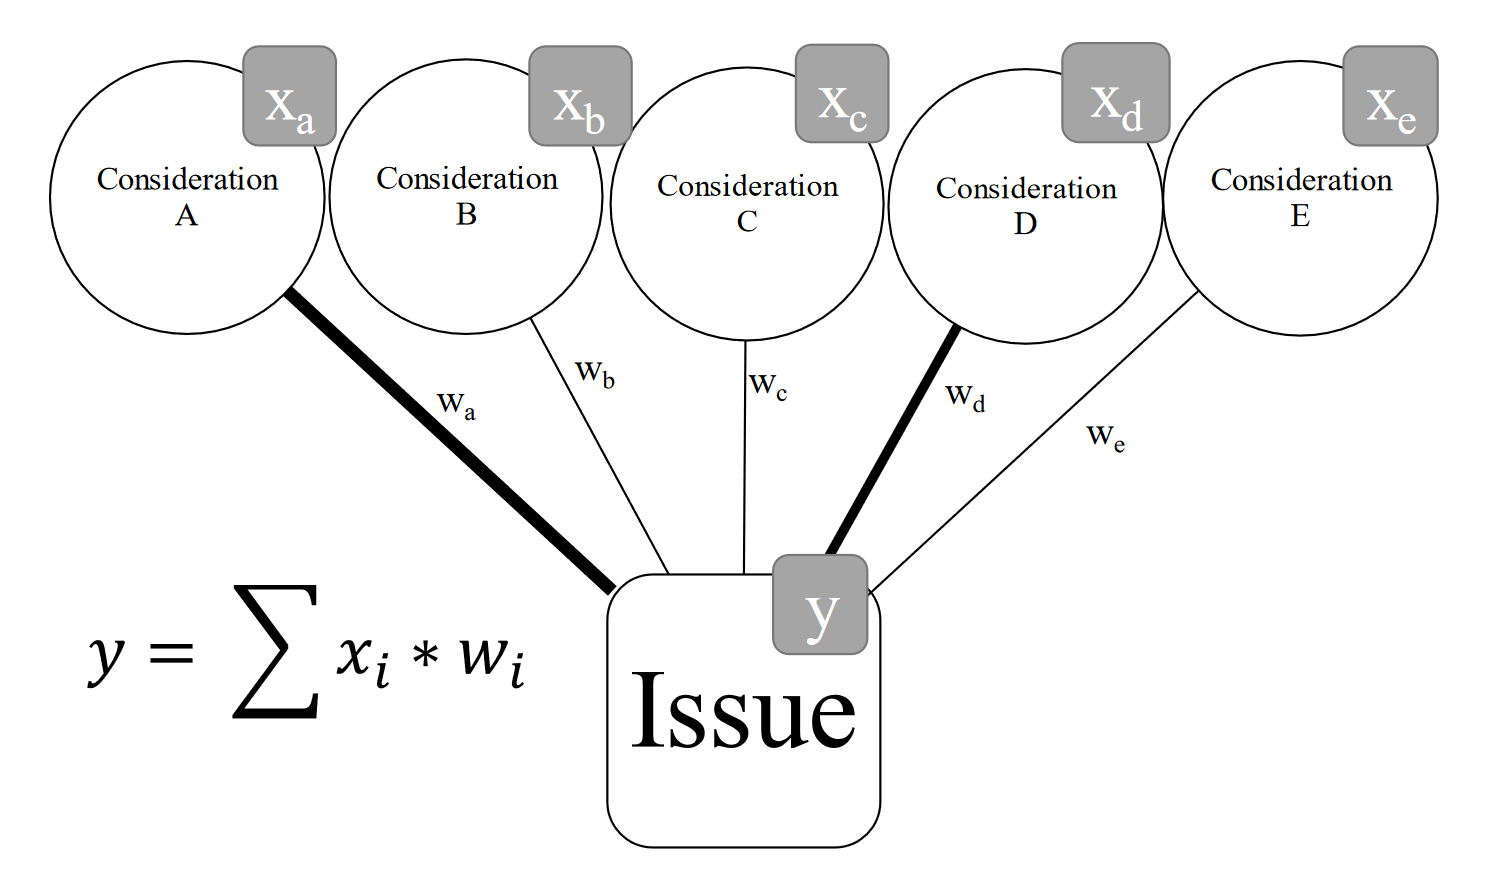
\includegraphics[width=\textwidth]{vis/CognitiveStorage.png}
    \caption{The cognitive evaluation of an issue $y$ is determined by the strength of association $w_i$ with other concepts with existing evaluations $x_i$.}
    \label{fig:cogStor}
\end{figure}

How does this model incorporate news content and other forms of political communication? News content can emphasize different considerations of an issue (``frames in communication''). By being exposed to the consideration, an individual's cognitive association of the issue at hand with the raised consideration strengthens (or in more technical terms: the weight of the consideration \(w_i\) increases). As a result, this specific consideration factors more prominently in the formulation of an overall attitude: ``media frames influence opinions by stressing specific values, facts, or other considerations, endowing them with greater apparent relevance to the issue than they might appear to have under an alternative frame'' (Nelson, Clawson, and Oxley 1997, 569).

Applying this to the issue of migration policy and the consideration of criminal migrants, one can imagine a news consumer confronted with an increased volume of news about crimes committed by migrants. The value-expectancy model predicts that i) the consumer forms a cognitive definition of migration that is increasingly associated with the issue of crime, meaning this consideration features more prominently when forming an opinion about the appropriate level of immigration; ii) as a result, their opinion about migration policies should become more restrictive, as the negative consideration of crime is weighted more heavily in the evaluation of the migration issue.

\medskip

\noindent \textit{\textbf{Association hypothesis}: When an individual is exposed more to a specific consideration about an issue, their association of the issue with this consideration should be strengthened.}

\noindent \textit{\textbf{Evaluation hypothesis}: When an individual is exposed more to a specific positive/negative consideration about an issue, their attitude about the overall issue should become more positive/negative.}

\hypertarget{framing-limits}{%
\section{Limits of Framing Effects}\label{framing-limits}}

Research on framing has shown for decades that citizens' attitudes and their issue associations are highly reactive to minor changes in the emphasis of specific considerations (Chong and Druckman 2007b, 2010; Druckman, Fein, and Leeper 2012; Kinder and Sanders 1990; Nelson and Kinder 1996; Nelson, Clawson, and Oxley 1997; Sniderman and Theriault 2004; for reviews see Busby, Flynn, and Druckman 2019; Druckman 2001; Leeper and Slothuus 2020). However, it remains unclear how well these experimental findings translate into citizens' everyday realities. Below, I outline three key assumptions in the generalization of experimental estimates.

First, taking experimental effects as estimates of the real-world impact of framing means making strong assumptions about citizens' exposure to frames: while framing studies usually simply present news articles or other forms of political content to respondents, news content in the real world competes with other news and entertainment content to reach its audience. Changes in news framing itself might affect how likely citizens are to consume news content: readers might be less likely to consume frames challenging their existing attitudes and reject news content containing such frames (and vice versa seek out attitudinally congruent information, Arceneaux and Johnson 2010; Druckman, Fein, and Leeper 2012). This process of `selective exposure/avoidance' (Bennett and Iyengar 2008), or a `confirmation bias' (Taber and Lodge 2006) brings with it a major endogeneity problem making purely correlational evidence rather uninformative. As most framing studies do not offer choice of content to respondents, engagement remains an assumption when taking experimental studies as evidence of framing effects in the real world (for an exception see Druckman, Fein, and Leeper 2012).

Second, even if consumers receive the content, it is not clear how much an individual relies on this source when forming an opinion on the subject. Information from different sources might `crowd out' the framing of one specific outlet: by consuming content from many sources, individuals give less attention to a given source, thereby severely limiting the overall impact of that outlet's coverage. Experimental evidence suggests that, when an individual receives competing frames, these cancel each other out, although the precise impact is dependent on the relative timing of exposure, the quality of the frame, as well as individual characteristics (Chong and Druckman 2007b, 2010, 2013). Additionally, individuals might update their perceptions slowly, as the increased emphasis of a consideration is not necessarily evident from the first few articles, instead arising from repeated exposure over time. Especially given that this study is concerned with a change in the \emph{relative} emphasis of a consideration, it might take some time for citizens' perceptions to catch up to the changing issue representation.

Third, cognitive engagement with frames might strongly differ in the real world compared to experimental contexts. Once individuals formed political attitudes, they might resist framing: Citizens presented with a plethora of news content about an issue will spend less time and cognitive energy on counter-attitudinal arguments than those supporting their viewpoint, lending more importance to considerations raised by amenable content (Taber and Lodge 2006). Experimental evidence suggests similar dynamics specifically for framing: when individuals are free to choose content, initial frames dominate the opinion-formation process, while novel frames are rejected (Druckman, Fein, and Leeper 2012) and even serve to strengthen pre-existing attitudes (Bechtel et al. 2015).

In sum, there are many reasons to assume that framing might have very different consequences in real-world environments than in their experimental emulations. If one takes experimental evidence as an approximation of the effectiveness of framing in the real world, they make many strong assumptions about citizens' exposure to, reliance on, and cognitive engagement with the frames in news content. Experiments can only incorporate few characteristics of the real world at a time. In order to test the external validity of framing effect studies, it is necessary to study observational data.

\hypertarget{research-design}{%
\section{Research Design}\label{research-design}}

In order to test whether changing news content affected political attitudes, I exploit an exogenously timed editorial change in the largest German newspaper, \emph{Bild}. As I will show, this editorial change resulted in a substantial shift in the papers' migration framing and is hence ideal to assess the effect of within-newspaper content shifts. The fielding of a large-scale panel survey in the same period allows to assess the precise impact of this change in news content on consumers' migration attitudes and related variables.

\hypertarget{a-rare-shift-in-migration-framing}{%
\subsection{A Rare Shift in Migration Framing}\label{a-rare-shift-in-migration-framing}}

In the summer of 2015, Germany became sanctuary for around 800,000 refugees who had fled war, violence, and famine in Syria and elsewhere. The German public debated how to deal with the newly arriving and for the first time since the post-war years, a radical right party was likely to win seats in the national parliament. Surprisingly, given its traditional populist style and right-wing takes on migration, the major tabloid newspaper \emph{Bild} initially maintained a somewhat balanced coverage of refugees, which -- although still portraying migrants more negatively than other outlets (Maurer et al. 2019) -- even started a campaign called ``\#RefugeesWelcome'' to gather support for the newly arriving\footnote{See \url{https://web.archive.org/web/20160114154402/https://www.bild.de/news/topics/fluechtlingshilfe/wir-helfen-buehne-42385428.bild.html}.}. This was often connected to chief editor Kai Diekmann, who hosted a refugee family in his home (Reichart 2015).

About one and a half years later, in December 2016, Axel Springer, the company owning \emph{Bild}, announced that Diekmann would leave the company. Less than a week after the announcement, it became public that prosecutors investigated Diekmann for sexual harassment. While the company claimed that this was not the reason for Diekmann's departure, the process might have been sped up as a result of the investigations\footnote{According to a former editor of the newspaper I talked to, rumors in the company at the time support this interpretation of events.} ({``{Springer-Mitarbeiterin wirft Diekmann Bel{ä}stigung vor}''} 2017). The migration coverage in \emph{Bild} severely changed when Diekmann left the newspaper in February 2017 and Julian Reichelt took over the position as editor-in-chief. The paper increasingly started painting a picture of refugees as criminals on the tabloid's front page (Niggemeyer 2018; Zudeick 2018). Headlines like ``I killed 40 people and want asylum'' increasingly dominated the migration coverage of the newspaper. In a speech months before he took over the position as chief editor, Reichelt outlined his motivation for such a shift in migration coverage: ``I can assure you: nothing has hurt {[}\emph{Bild}{]} economically as much as our clear, humane, empathetic stance in the refugee crisis'' \footnote{Reichelt in a speech at Deutschlandfunk's conference "Formate des Politischen 2016": \url{https://vimeo.com/190347766}}. While he expressed his support for the decision to take this stance at the time, he argued that the German media shows too little tolerance towards anti-immigration attitudes, thereby excluding those holding such views from political discourse.

This case presents a unique opportunity to study the effects of media content on public opinion. As I will show below, the emphasis of crime strongly increased in \emph{Bild}'s migration coverage following Reichelt's takeover. The change of editor itself was not discussed in the media, which means any opinion changes among readers can only be the result of the changing content (see Spirig 2020). Additionally, the timing of the editorial change is likely exogenous, given the pressure from allegations against Diekmann. In summary, \emph{this case is as close as possible to a field experiment in which a specific consideration of migration coverage is amplified in the coverage of one newspaper, but not others}.

In the following sections, I will outline a framework for the measurement of emphasis frames in communication and showcase the increasing emphasis of crime in \emph{Bild}'s migration coverage. Subsequent sections will describe the panel data and variables to measure frames in thought (namely migration attitudes and their association with attitudes about crime) and define the difference-in-difference estimator. I will close with a discussion of the expected experimental effect size and the minimal effect size of interest to provide baselines for comparison of the estimator.

\hypertarget{measuring-frames-in-communication}{%
\subsection{Measuring Frames in Communication}\label{measuring-frames-in-communication}}

To measure migration framing in the news, I collected 2.5 million newspaper articles from the websites of the most important German broadsheets \emph{Frankfurter Allgemeine Zeitung (FAZ), Spiegel Online (SPON), Süddeutsche Zeitung (SZ), Die Tageszeitung (TAZ), Die Welt}, as well as \emph{Bild} for the period 2013-2019. These outlets reach a substantial share of the German public, with \emph{Bild} distributing over 1.7 million print copies and registering over 550 million web impressions at the time (see section 2.1 in the online appendix for more information). Following the value-expectancy model, I identify crime frames in migration coverage in a two-step process: first, I identify content about migration. Second, I identify content about crime \emph{within} migration coverage. This approach closely resembles the value-expectancy model outlined \protect\hyperlink{framing-effects}{above}, as I first identify coverage about the \emph{issue}, before identifying the \emph{consideration} emphasized in the discussion of this issue.

To identify whether an article is about migration, I employ supervised machine learning. As migration content is rare, and sufficient training data needs to be available to train functional classifiers, articles cannot be selected randomly for annotation\footnote{If migration content made up about 3 percent of all articles and the sample were selected randomly, one would find around 30 migration articles per 1000 articles, which provides rather limited information about the class of interest and results in worse recall of the classifier, as the best guess in highly imbalanced data is simply the most common outcome.}. Instead, I take a more informed approach by oversampling articles which are likely about migration: after constructing a seed dictionary of migration-related terms, I apply dictionary extension using German GloVe word-embeddings\footnote{Downloadable from \url{https://deepset.ai/german-word-embeddings}.} to construct a comprehensive dictionary, and apply it to the articles\footnote{The dictionary can be found in online appendix 2.2.1.}. Based on the relative share of migration words in an article, I draw a stratified sample of 300 articles (100 from articles with no migration terms, 100 from the quarter with the highest share of migration terms and 100 from the remaining articles with relative frequencies of migration-related terms in between these two groups) for each newspaper for a total of 1,800 papers. Then, a coder hand-coded these articles, assessing whether their main topic is related to migration\footnote{The coder was instructed to annotate articles referring to migration or integration, which includes discussions of refugee numbers, immigrants' and naturalization rights, and general reports of migration. More information can be found in online appendix 2.2.3.}.

Using this sample, a BERT transformer model\footnote{\url{https://huggingface.co/bert-base-german-cased}}, pre-trained on a large German corpus of Wikipedia articles, News, and legal documents, is fine-tuned on a random subset of 1,400 annotated articles (training set) with a validation set of 200 articles. After fine-tuning, the model correctly classifies 95.5\% of a test set of 200 articles (F1: 0.94, recall: 0.93, precision: 0.95). This classifier is then used to annotate all 2.5 million newspaper articles. For the period from 2013 to 2019, around 90,000 articles (3.6\%) are identified to treat the issue of migration\footnote{A precise description of the classification process for migration and crime-related articles, including sampling dictionaries, instructions for coders, and preprocessing steps, can be found in online appendix 2.2.}.

To identify migration coverage containing the crime consideration and thereby associating migration with crime, I first fine tune a BERT classifier for German language in a similar fashion as above, this time with coverage about crime as the outcome of interest. Using a training set of 1400 articles (selected using the identical process as above), a validation set of 200 and a test set of 200 articles, the classifier reaches a very good performance with an F1 score of 85.7\%. I then apply this classifier to the approximately 90,000 articles about migration identified by the first classifier. About 7\% of all migration coverage consists of articles about some form of crime\footnote{See online appendix 2.2.7 for more information.}.

The left panel of figure \ref{fig:treatment} shows the share of migration coverage devoted to crime news, once for \emph{Bild} (solid, black line) and once for all other newspapers (dashed, gray line). As we can see, \emph{Bild}'s attention to crime news in its migration coverage substantially increased directly following the takeover of Julian Reichelt, while it focused less on the issue preceding the editorial change\footnote{Note that this data consists exclusively of original Bild content. Treatment estimates including third-party authored content are similar in size. For a more extensive discussion see online appendix 2.2.5.}. The trends run parallel to each other preceding the treatment. The lower attention to crime in 2015 and the increase in 2016 is in line with prior research (Maurer et al. 2019). The right-hand panel shows difference-in-difference estimates of the crime emphasis in migration coverage of one newspaper compared to all others, before and after the editorial change in \emph{Bild}. One can see that \emph{Bild} was the only newspaper which substantially changed its emphasis of the frame, increasing the share of articles devoted to crime by around 5 percentage points (over 40 percent percent of the pre-treatment average), while other newspapers maintained their levels of attention.

\begin{figure}[!ht]

{\centering 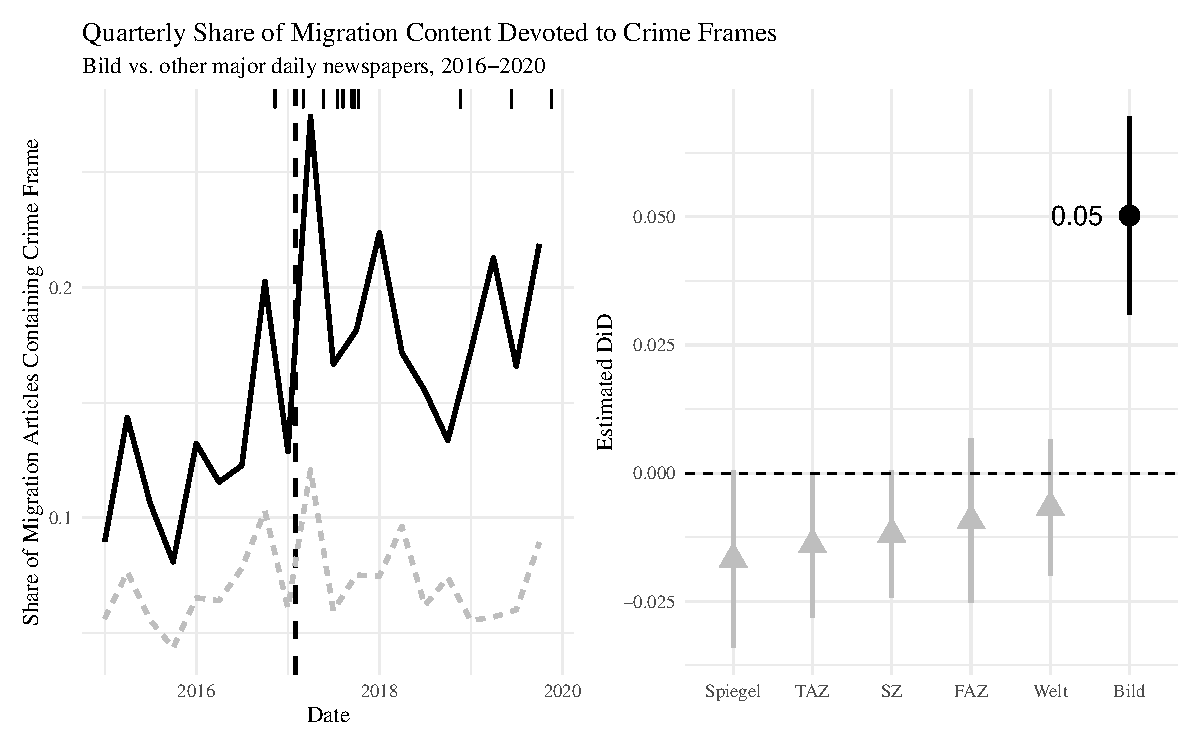
\includegraphics{Manuscript_Framing_files/figure-latex/treatment-1} 

}

\caption{Estimated change in attention to crime content in migration coverage, Bild vs. other newspapers. Black ticks in left panel indicate survey waves.}\label{fig:treatment}
\end{figure}

\hypertarget{measuring-frames-in-thought}{%
\subsection{Measuring Frames in Thought}\label{measuring-frames-in-thought}}

In order to assess the impact of this change in framing on public opinion, I need data on citizens' immigration attitudes, as well as their news consumption. The 2017 Election Panel by the German Longitudinal election study contains this data. It consists of a total of 15 waves from 2016-2020, with 10,000 -- 20,000 respondents per wave (Debus, Faas, and Roßteutscher 2017). Thirteen of these waves contain questions on immigration attitudes, asking respondents whether immigration of foreigners should be liberalized or restricted. Responses were recorded on a seven-point Likert scale. This variable was centered on zero (\(-3\) -- liberalize, \(3\) -- restrict; the precise wording in the survey can be found in online appendix 1.1.2).

To measure exposure to \emph{Bild} news, I use a question on newspaper consumption. The question provides respondents with a list of the six major daily newspapers plus an option ``another daily newspaper'' and asks whether they had consumed the paper in print or read articles from their website, and if so, how many days in the past week. Readers are defined as \emph{treated} if they indicate to read \emph{Bild} in the pre-treatment wave and as \emph{untreated} if they indicate not to read the tabloid in the pre-treatment wave, nor any subsequent wave\footnote{See online appendix 1 for descriptives of all mentioned variables.}.

In order to assess the effect on the association of immigration and crime, I also measure attitudes about crime using an item asking whether the governments' capabilities to fight crime should be extended\footnote{Precise question wording: "State powers to fight crime should be expanded, even if this means more surveillance of citizens."} on a 5-point Likert-scale. I also use additional dependent variables assessing attitudes about the need for immigrants to integrate into German culture (7-point scale), mentioning immigration as the most important problem (binary indicator), and a thermometer score for the radical-right \emph{AfD} (10 point scale).

\hypertarget{estimation}{%
\subsection{Estimation}\label{estimation}}

To assess the precise impact of increased attention to crime in migration coverage, I will present evidence from a \emph{difference-in-differences} (DiD) estimator to show the effect of the editorial change -- and the related content shift -- on migration attitudes:

\[
y_{iw} = \alpha + \beta_1*Post_w + \beta_2 * Post_w * BildReader_i + \phi_w + \rho_i + \epsilon_{it} 
\]

The dependent variable \(y_{iw}\) indicates respondent \(i\)'s migration attitude in a given survey wave \(w\), measured on the Likert scale described above. The conditioning variable \(BildReader_i\) is a simple binary variable indicating whether respondents read \emph{Bild} in the past week and is measured in the pre-treatment wave. \(Post_w\) indicates whether an interview took place preceding or following the editorial change. The estimator of interest is \(\beta_2\), which indicates the change in migration attitudes of \emph{Bild} readers following the editorial change, controlling for time-constant (\(\rho_i\)) and wave-specific (\(\phi_w\)) factors with fixed effects, as well as general pre-post shifts in migration attitudes (\(Post_w\)). Note that the pre-treatment differences of treatment and control group are corrected for in the individual fixed effects, as the groups are constant over time (readership is only assessed pre-treatment). As the panel data contains only one pre-treatment wave, the parallel trends assumption cannot be tested with this data directly, but assessing the trends using the GLES Longterm Panel (Roßteutscher et al. 2018) shows that \emph{Bild} and non-\emph{Bild} readers' immigration attitudes move in parallel preceding the treatment (see online appendix 3.1).

\hypertarget{expected-effect-size}{%
\subsection{Expected Effect Size}\label{expected-effect-size}}

To provide a baseline expectation regarding the effect size in experimental work, it is useful to consider an expected effect size at this point. Despite the abundance of framing effects studies, there is no common standard to assess the magnitude of framing effects. Even the correct measurement of the magnitude is a contested question, as different control groups can be compared (Druckman 2001; Chong and Druckman 2007c, 109f for a discussion). Additionally, framing effects differ based on the polarization and salience of the issue (Lecheler, De Vreese, and Slothuus 2009), repeated exposure (Chong and Druckman 2007a), the sender (Slothuus and De Vreese 2010), political knowledge (Chong and Druckman 2007b), as well as the reference of certain groups (Nelson and Kinder 1996). Generally, reported effect size around 30\% of the scale are not uncommon (Slothuus and De Vreese 2010), sometimes even over 40\% (Chong and Druckman 2007c, 104), but most results lie in between 10\% and 25\% of the scale when comparing opposing frames pushing respondents in opposite directions\footnote{As many studies do not include a control group receiving no frame, this is the most comparable metric.} (Lecheler, De Vreese, and Slothuus 2009; Nelson, Oxley, and Clawson 1997; Nelson, Clawson, and Oxley 1997; Slothuus 2008; Slothuus and De Vreese 2010).

As experimental treatments are likely designed in order to elicit strong responses, and given biases towards null effects in the production of scientific knowledge (see e.g.~the recent debate regarding nudging effects: Maier et al. 2022), reported effects likely display a selection bias towards strong treatments. The treatment in the present study can be considered rather strong, as the crime consideration is associated with a strongly negative evaluation and the relative increase in the prevalence of this content is large \footnote{5 percentage point increase compared to pre-treatment share of 11.8 percent in Bild, an over 40 percent increase.}. Given these considerations, I expect an effect of around 10\% of the scale, or 0.6 on the seven-point scale\footnote{As the scale runs from one to seven, it spans six points wide.}, which represents a conservative estimate compared to reported experimental effects. At this point, it should be mentioned that it is rather difficult to compare these experimental effects with a real world treatment. Experiments expose participants to one of two potential considerations, whereas in the real world, newspapers can only increase the relative prevalence of a given consideration.

As suggested by Lakens (2017), I also compare the estimated effect to equivalence bounds indicating the smallest effect size of interest (SESOI) in order to provide a baseline for a meaningful effect size. I define the SESOI at a 2.5\% change, or 0.15 on the seven-point scale, which represents a fraction of the conservative experimental estimate and sets a fairly low bar given the strong treatment. This SESOI can be used to define equivalence bounds. Any effect estimated to lie within these bounds with statistical significance (i.e.~a 95\%-confidence interval in-between the positive and negative effect of this size) is too small to constitute a meaningful effect, as the hypothesis that the effect reaches any size of interest can be rejected (see also Peyton 2020).

\hypertarget{results}{%
\section{Results}\label{results}}

I will first present evidence describing the effect on immigration attitudes and the association of immigration with crime attitudes. Then, I will assess the impact across time and on related variables to inspect the robustness of the estimation. The last section will trace the key assumptions in the generalization of experimental estimates discussed in the \protect\hyperlink{framing-limits}{section on the limits of framing effects}.

\hypertarget{effect-on-migration-attitudes}{%
\subsection{Effect on Migration Attitudes}\label{effect-on-migration-attitudes}}

According to the expectancy-value model, the most direct implication of increased exposure to crime frames in migration coverage should be a more restrictive attitude concerning immigration. The upper panel of figure \ref{fig:singleplot} plots the average immigration attitude among \emph{Bild}-readers compared to those never reading \emph{Bild}. The dashed vertical line indicates the timing of the change of the editor-in-chief at \emph{Bild}. Higher values indicate more restrictive migration attitudes. We can see that \emph{Bild} readers generally hold more restrictive immigration attitudes with a difference of about 0.4 on the seven-point scale. Both trends move largely parallel and seem to react to shocks similarly.

The lower panel of figure \ref{fig:singleplot} visualizes the average treatment effect, based on the model described in the \protect\hyperlink{estimation}{estimation section}. Dashed vertical lines indicate the expected effect from the experimental literature. The dotted lines indicate the equivalence boundaries/SESOI. The model suggests a clear null effect. This effect is not significantly different from zero, but significantly smaller than the above-defined SESOI of 0.15 on the seven-point Likert scale. The point estimate indicates a 0.019-point change among \emph{Bild} readers following treatment (\emph{t =} 1.33, \emph{p =} 0.22). This represents only a fraction (3.1\%) of the already conservative experimental estimate of 0.6. The finding is robust to different model specifications, as well as using data from the GLES Longterm Panel (see online appendix 3.2 and 3.4).

\begin{figure}[!ht]

{\centering 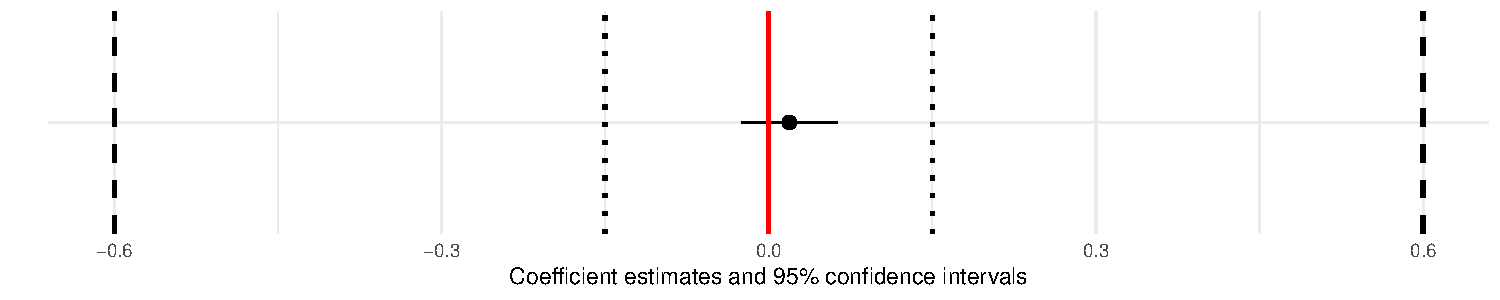
\includegraphics{Manuscript_Framing_files/figure-latex/singleplot-1} 

}

\caption{Top Panel: Development of Migration Attitudes across Time, by Bild-Readership. Bottom Panel: Average Treatment Effect.}\label{fig:singleplot}
\end{figure}

\hypertarget{effect-on-the-association-of-crime-and-migration-attitudes}{%
\subsection{Effect on The Association of Crime and Migration Attitudes}\label{effect-on-the-association-of-crime-and-migration-attitudes}}

Framing theory suggests that increased exposure to a specific consideration about an issue also leads to stronger association of the issue with this consideration. In the present case, this should mean that the correlation of attitudes on immigration with attitudes about crime should increase. The GLES Panel data contains a variable asking respondents whether ``the state's capabilities to fight crime should be extended, even if that would entail more surveillance'', asked in three waves overlapping with the migration attitude question.

Figure \ref{fig:corplot} shows the bootstrapped correlations of crime- and migration attitudes in treatment (\emph{Bild}-readers in pre-wave) and control group (never \emph{Bild}-readers), for each wave. The lines indicate the mean estimate, while the whiskers indicate the upper and lower 95\%-confidence interval, as defined by the 2.5 and 97.5 percentiles of the distribution of bootstrapped estimates. The dotted line indicates the counterfactual development, assuming that \emph{Bild}-readers behaved similar to the general population not reading \emph{Bild} in the absence of a change in migration framing. Surprisingly, the association of crime and immigration attitudes is initially weaker among \emph{Bild} readers. Nevertheless, the treatment group actually saw a \emph{smaller} increase in the correlation of crime and migration attitudes in the first post-treatment wave than the control group. The difference-in-differences in correlations of -0.028 is substantively rather small (9.3 percent of the average pre-treatment control group correlation) and not significantly different from zero with a bootstrapped 95\% confidence interval of {[}-0.079, 0.022{]}. In the last wave, the association decreases less than in the control group but the difference-in-differences does not reach conventional levels of significance compared to the pre-treatment wave (0.035, {[}-0.029, 0.094{]}). The association of crime and immigration attitudes did not increase among \emph{Bild} readers, relative to the control group.

\begin{figure}[!ht]

{\centering 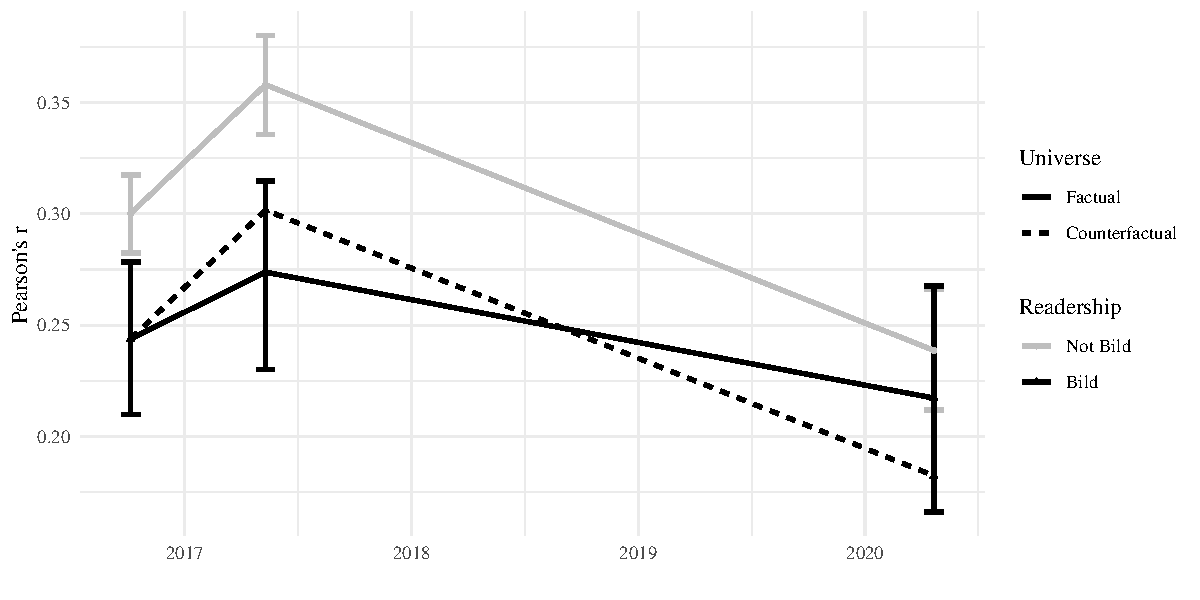
\includegraphics{Manuscript_Framing_files/figure-latex/corplot-1} 

}

\caption{Correlation of crime and migration attitudes in treatment and control group, pre- (wave 1) and post-treatment (waves 3 \& 13).}\label{fig:corplot}
\end{figure}

Following (Nelson and Kinder 1996), I also regress immigration attitudes on attitudes towards crime and investigate whether this association changes as a result of the change in coverage. Similar to the differences between the groups, I find a weaker association among readers of the tabloid, but no significant or substantively large difference post-treatment or when interacted with the DiD-term (see table in online appendix 3.5). Respondents do not associate crime more strongly with migration following the change in migration coverage in \emph{Bild}.

\hypertarget{effect-on-alternative-dependent-variables}{%
\subsection{Effect on alternative dependent variables}\label{effect-on-alternative-dependent-variables}}

While opinions about immigration and their association with attitudes about crime remain unaffected, it might well be that an increased exposure to crime framing affects other variables. For example, increased attention to crime within migration coverage might increase individual perceptions of the importance of migration, or raise concerns about the integration rather than the immigration of migrants. Similarly, support for the radical-right \emph{AfD} as owner of the migration issue could increase as a result of increased exposure to this type of migration coverage.

Figure \ref{fig:multidv} displays standardized effects of the change in newspaper framing on immigration attitudes (for reference) and three related dependent variables, namely integration attitudes, the likelihood to report migration as the most important problem facing the country, as well as thermometer scores for the radical-right AfD (see online appendix 1 for precise variable descriptions). To provide reference values again, I rescale the expected experimental effect of 0.6 and SESOI of 0.15 for immigration attitudes to standard deviations. This results in baselines of 0.34 and 0.08 standard deviations, which can be considered fairly small. All estimated effects are significantly smaller than the SESOI and all associated 95\%-confidence intervals contain zero. This means we can reject the hypothesis of meaningful effect size, but cannot reject that the estimate is statistically different from zero. All estimates suggest a clear null effect.

\begin{figure}[!ht]

{\centering 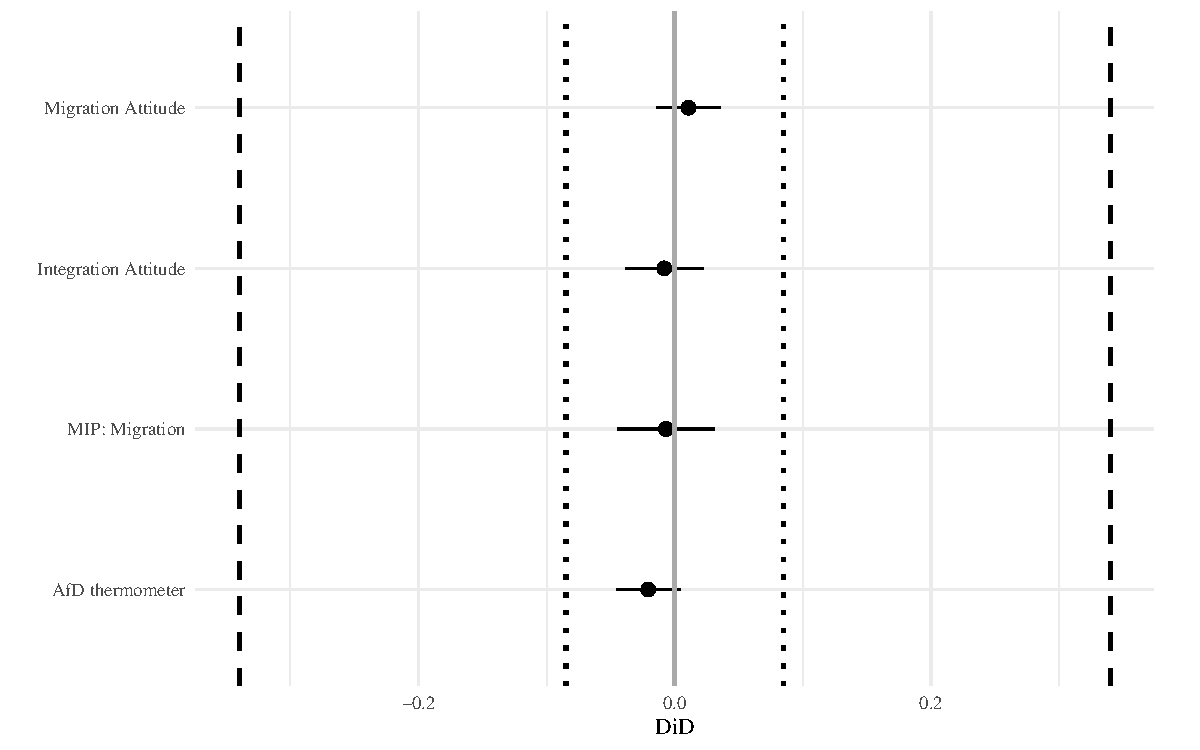
\includegraphics{Manuscript_Framing_files/figure-latex/multidv-1} 

}

\caption{Standardised effect of change in framing on alternative dependent variables. Dotted vertical lines indicate minimal relevant effect (0.2 SD). Full models available in online appendix 3.3.}\label{fig:multidv}
\end{figure}

\hypertarget{explanations-for-resistance-to-framing}{%
\subsection{Explanations for Resistance to Framing}\label{explanations-for-resistance-to-framing}}

Although mounting experimental evidence suggests large effects of framing in the experimental context, I find robust evidence that a substantial increase in the emphasis of crime in migration coverage did not affect immigration attitudes, their association with crime, or any related variables. As outlined above, there are several key assumptions in the generalization of framing effects from experimental contexts. First, those witnessing a changing news framing might select out of the treatment instead of changing their attitudes. Second, if citizens consume many sources of political news at the same time, they might not react to a change in a single news outlet. Third, repeated exposure over time might produce effects which are not perceptable in earlier waves. Fourth, issue attitudes might only be responsive to news framing during critical periods of politicization. The following section presents evidence about each of these assumptions.

\hypertarget{selective-exposure}{%
\subsubsection{Selective Exposure}\label{selective-exposure}}

As the migration framing in \emph{Bild} becomes more conservative, this could also lead readers with more liberal migration attitudes to stop reading the newspaper, as they avoid information challenging their views. If readers selectively exposed themselves, I expect that the share of those holding liberal views about immigration reading \emph{Bild} would drop more significantly than other reader's share, as they actively select out of the newspaper. That is not the case: Liberals' and conservatives' share of readers track each other closely, with those reporting liberal migration attitudes in the first wave even reporting to read Bild at \emph{higher} shares than conservatives in later waves (see figure \ref{fig:selectionPlot}). What is interesting is that those reporting neutral migration attitudes seem to be more inclined to leave the newspaper: Neutral readership declines to a level of 57\%, around 5 percentage points below the share reported by liberals (62\%) and 3pp below the level of conservatives (60\%). Regressing individual choice to read \emph{Bild} in later waves on initial reported migration attitudes within the subsample of initial \emph{Bild} readers shows a 5\% lower chance to report Bild readership among initial neutral readers, compared to liberal readers (\(p =\) 0.003), whereas there is no significant or substantial difference for conservative readers. Surprisingly, \emph{Bild} readers reporting centrist immigration attitudes select out of the newspaper at higher rates than both conservative or liberal readers, whereas there is no significant difference between the latter two. I also tested whether the association of reading the newspaper and conservative immigration attitudes was streangthened over time. As online appendix 3.6.1 shows, there is no evidence of this process either.

\begin{figure}[!ht]

{\centering \includegraphics{Manuscript_Framing_files/figure-latex/selectionPlot-1} 

}

\caption{Share of initial Bild readers reporting readership in later waves by initial migration attitude. Dashed vertical line indicates editorial change.}\label{fig:selectionPlot}
\end{figure}

\hypertarget{crowding-out}{%
\subsubsection{Crowding Out}\label{crowding-out}}

If readers did not avoid persuasive content by selecting out of the outlet, how can the absence of a framing effect be explained? A second possibility is that readers are exposed to so many other sources of political information that the change in the framing of a single outlet does not severely affect their attitudes. If that were the case, consumers with a less diverse news diet would still receive a larger relative share of their information from a single outlet and hence respond to changes in the framing of this outlet. In other words, I expect a heterogeneous treatment effect: those with very limited news diets should experience an attitudinal change, whereas this effect should decrease with increasing exposure to other outlets. The panel data used in this study contains a number of variables that allow me to measure the diversity of a respondent's news diet. Respondents could indicate on how many days they consumed newspapers other than \emph{Bild} in the preceding week. Summing these responses allows to generate a variable indicating how many newspapers other than \emph{Bild} have been consumed, weighted by the intensity of their readership (see online appendix 1.2.3 for a detailed description).

Results suggest a precise null effect of 0.006 {[}-0.05; 0.062{]} within the group of those consuming no other newspaper, which is about 1\% of the expected experimental baseline and much smaller than the SESOI of 0.15. The estimate is virtually identical for respondents indicating to consume other newspapers 1-3 times per week. Point estimates for other groups (consuming other newspapers 4-9, 10-15 or more than 15 days\footnote{A 'day' refers here to the additive days for every mentioned newspaper, that means if an individual reads newspaper A for seven days and another for six days, the total number of days will add up to thirteen.} in the preceding week) are well below the SESOI and statistically not different from zero, although estimation is less precise with higher values\footnote{See online appendix 3.6.2 for a visualization of all effects described in this section.}.

I also exploit available data on consumption of political news from TV news providers (binary indicator) and on how many days respondents informed themselves about politics on the internet. Effects in the group of those indicating to have not consumed TV news (or their online counterparts) show a similarly precise null effect (-0.073 {[}-0.167; 0.021{]}). The estimate among those not informing themselves about politics on the internet is less precise, neither being significantly different from the SESOI nor zero, however the magnitude of the point estimate of 0.079 is about half of the minimal effect size of interest. No clear pattern emerges with increasing internet exposure, in fact the only significant (but tiny) positive effect of 0.164 ({[}0.054; 0.273{]}) is observed in the group consuming political news on the internet on one out of seven days in the past week.

\begin{figure}[!ht]

{\centering \includegraphics{Manuscript_Framing_files/figure-latex/crowdout-1} 

}

\caption{Heterogenous treatment effects by level of exposure to different news sources.}\label{fig:crowdout}
\end{figure}

Crowding out does not explain the absence of an effect of news framing on political attitudes. Those respondents consuming no other political information from newspapers, TV news, or online sources are no more reactive to a change in migration framing than those with a more diverse news diet.

\hypertarget{slow-updating}{%
\subsubsection{Slow Updating}\label{slow-updating}}

If readers only perceive the change in content across longer time periods, the effect should slowly unfold over time. Then, initial absence of change might bias the estimates downward and thereby mask an effect. To assess whether an effect develops over time, figure \ref{fig:migwaves} assesses the effect within split-samples for each post-wave compared to the pre-treatment wave. This allows the assessment of heterogeneous treatment effects across time. The black dots with associated confidence intervals indicate the estimated effect for each wave. The horizontal dashed line indicates the expected effect based on experimental evidence (0.6), whereas the dotted horizontal line indicates the SESOI of 0.15. The vertical dashed line indicates the timing of the editorial change. Over the course of the entire year 2017, the effect is clearly smaller than the SESOI, and includes zero. However, estimates for waves 10 and 11 in late 2018 and mid-2019 -- more than one and a half years after the editorial change -- showcase effects statistically different from zero, and including the SESOI boundary. The effects are rather small, with a point estimate of 0.09 on the seven-point Likert scale, as well as an upper boundary just above the SESOI at 0.162. The waves in late 2019 and early 2020 return to point estimates at slightly lower levels (0.067, 0.074), with confidence intervals including zero. While there is evidence of persuasion in the long term, the effect size is overall very small.

\begin{figure}[!ht]

{\centering 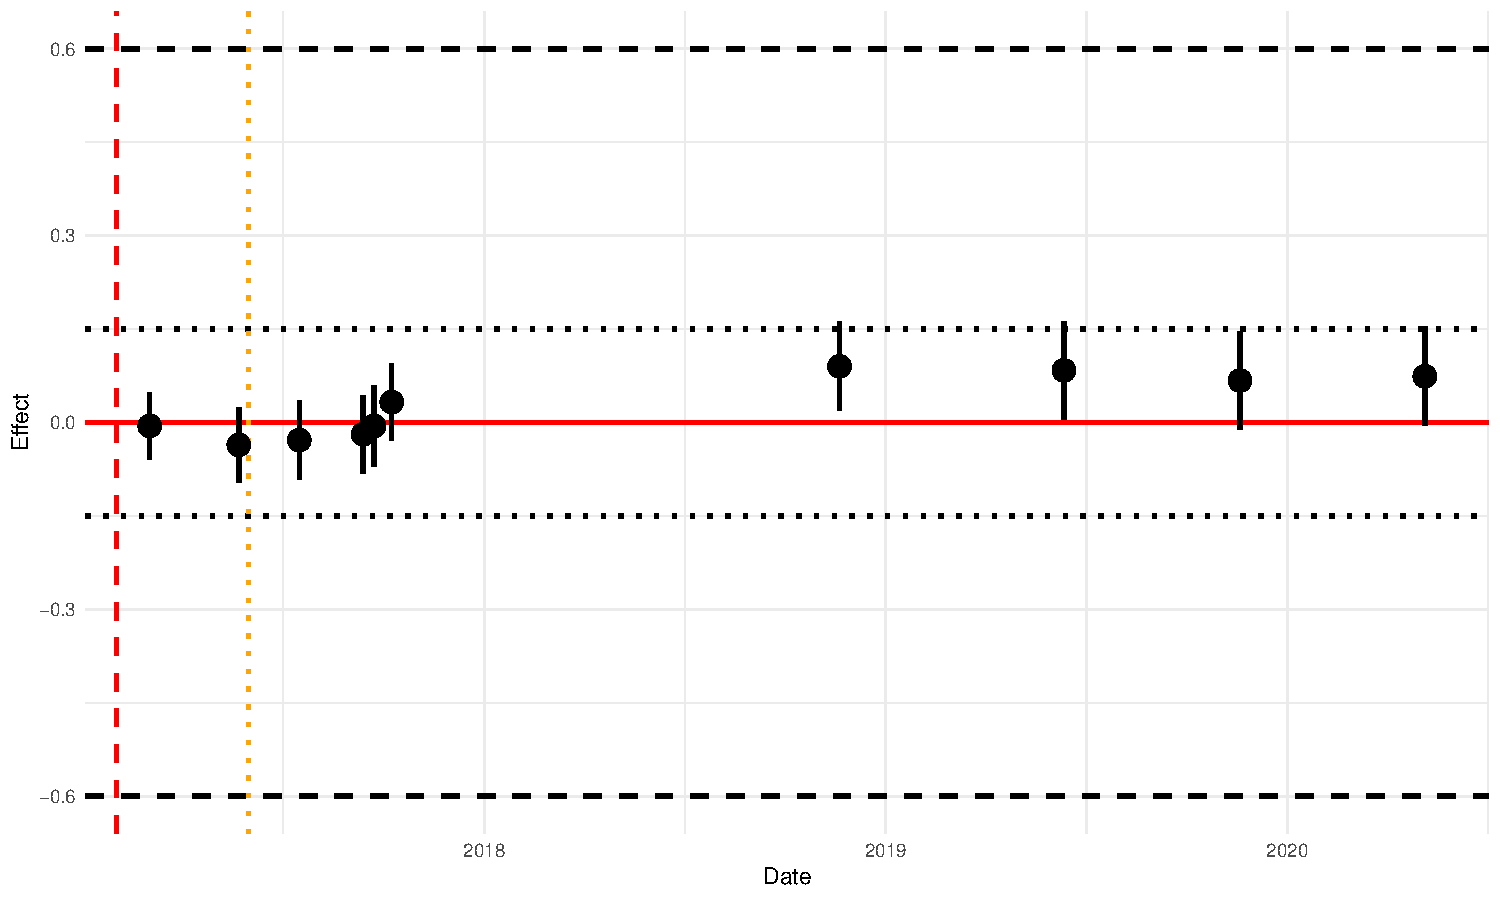
\includegraphics{Manuscript_Framing_files/figure-latex/migwaves-1} 

}

\caption{Effect on migration attitudes, by survey wave.}\label{fig:migwaves}
\end{figure}

\hypertarget{attitude-crystallisation}{%
\subsubsection{Attitude Crystallisation}\label{attitude-crystallisation}}

\begin{figure}[!ht]

{\centering \includegraphics{Manuscript_Framing_files/figure-latex/MigChange-1} 

}

\caption{Change in individual immigration attitudes 2014-2018. Data taken from the GLES Longterm Panel (Roßteutscher et al. 2018).}\label{fig:MigChange}
\end{figure}

Readers did not react by selecting out of the newspaper, nor was the change in framing crowded out by other sources of information. Even long-term exposure produced rather minor effects. Another possible explanation for this resilience to framing is that individuals informed themselves about the issue and formed an attitude once the issue emerged, in this case in 2015 during the large migratory movements in Europe. If that were the case, opinions should change more in 2015 than the following period. Figure \ref{fig:MigChange} shows this statistic using GLES Longterm Panel data (Roßteutscher et al. 2018). Unfortunately, I lack data for the period preceding 2014 and the year 2015, forcing me to make one-off comparisons rather than providing a longitudinal picture. The left panel compares the absolute change in individual immigration attitudes from 2014-2016 and 2016-2018, always measured in January. That is, if a respondent held an attitude of 3 (leaning conservative) on the ten-point scale in 2014 and moved to 2 in 2016, the absolute change would be equal to 1. Immigration attitudes in the GLES sample shifted on average by a substantial 2.25 from 2014 to 2016 (lower 95\% confidence interval 2.19, upper 2.3), while they shifted significantly less in the period 2016-2018 (1.73; {[}1.69 1.78{]}). The right-hand panel shows the change across one year, comparing 2016-2017 to 2017-2018 (to be comparable, the periods have to be of equal size). Across the course of 2016, when the German public debated the integration of refugees and the events of new years eve 2016 in Cologne, individuals still display higher levels of attitudinal change (1.74; {[}1.69 1.79{]}) than 2017-2018 (1.54; {[}1.5 1.59{]}).

Although we lack evidence about the changes in migration attitudes pre-2015, these substantial and significant differences (technically differences-in-differences) suggest that, during the politicization of the issue in 2015, citizens updated their attitudes about the immigration issue, which, after the debate cooled down, crystallized into stable attitudinal positions, resistant to additional information.

\hypertarget{conclusion}{%
\section{Conclusion}\label{conclusion}}

What are the limits of media power? While the answer to this question has profound implications for our understanding of elite influence in contemporary democracies, we currently lack evidence about the scope conditions of media effects. This study addresses this gap by presenting evidence from a rare shift in the migration coverage of Germany's largest tabloid, \emph{Bild}. The presented results are robust evidence that readers' immigration attitudes remained surprisingly unaffected. Estimates of attitudinal change are indistinguishable from zero and remain below minimal effect sizes in a number of specifications, dependent variables, and subgroups.

The paper presents a clear explanation for this resilience. After ruling out that readers selected out of the newspaper or that exposure to other sources conditions the effect, I find support for the explanation that attitudes became unresponsive after 2015: following this period, the average change in individual immigration attitudes decreased substantively and significantly. This suggests that the newspaper has missed a critical window to influence readers' immigration attitudes.

This finding relates to a broader experimental literature on the persuasiveness of information under different degrees of societal salience and politicization. Arceneaux and Kolodny (2009) find that campaign messages can affect political attitudes, but only on issues which are not politicized. They conclude: ``{[}p{]}eople's attitudes on these types of issues are likely to be crystallized and firm, limiting the effect of persuasive communication'' (Arceneaux and Kolodny 2009, 245). Lecheler, De Vreese, and Slothuus (2009) study this question regarding framing effects, comparing high- and low-importance issues, and show that only the latter are responsive to framing. This finding has been reproduced in realistic settings involving opposing party cues (Bechtel et al. 2015) and research about the impact of pre-treatment and exposure to conflicting frames point in similar directions (Druckman and Leeper 2012; Druckman, Fein, and Leeper 2012).

While this evidence might seem like a contradiction to the idea that attitudes change \emph{most} during the politicization of an issue, it is useful to take a longitudinal perspective. The model I propose views political issues as defined in public discourse. Once an issue emerges in public debate (usually because of an external event), problem definitions, causal explanations, and potential solutions are collectively debated. Political actors struggle to get their frames considered. Only a small subset of these frames will get to dominate public debate, shaping citizens' understanding of the issue. This collective definition will be resistant to attempts of framing and thus stabilize attitudes. Attitudinal change accelerates during the politicization of an issue, as citizens update their perceptions. Once a stable collective issue definition emerges, individuals become resistant to further information about the issue.

This model also speaks to a large body of media effects research. It suggests that the power of the news media to shape public opinion is more limited than previously thought. Even when elites try, they might not always be able to manipulate their audience's political attitudes. While studies on media effects have shown that public opinion \emph{can} be affected by changing news exposure (DellaVigna and Kaplan 2007; Foos and Bischof 2022; Grossman, Margalit, and Mitts 2022; Levendusky 2022), this study took a first step to investigate under which conditions this process takes place.

This study has several limitations, which should be addressed by future research. The argument in this paper applies to liberal democracies in general, but I present evidence from Germany, which is a Western European democracy with a relatively high-quality press, large public broadcasters, and a moderately involved electorate. While the experimental evidence from the US, Switzerland, and Denmark discussed above supports the idea that this might be a more general phenomenon, future observational studies should assess longitudinal panel data in other contexts. Similarly, migration might be a `special' issue, meaning that citizens form attitudes differently on this issue (Kustov, Laaker, and Reller 2021). Lastly, my analysis of the `crystallization' of attitudes is limited by the available data. To observe the ac- and deceleration of attitudinal change relative to issue's politicization, future research should exploit panel data from different contexts and on different issues, but ultimately more longer-term panel data tracking issue attitudes will be necessary. This is especially challenging, as attitudinal measures are usually added to survey questionnaires only \emph{after} the politicization of these issues. However, to get a full picture of the process of attitude formation, it is necessary to track the same issues irrespective of their current relevance in day-to-day politics. Otherwise, researchers will only observe issue attitudes after the relevant processes of attitude formation have taken place.

\pagebreak

\hypertarget{resources}{%
\section*{Resources}\label{resources}}
\addcontentsline{toc}{section}{Resources}

\hypertarget{refs}{}
\begin{CSLReferences}{1}{0}
\leavevmode\vadjust pre{\hypertarget{ref-Ajzen2000}{}}%
Ajzen, Icek, and Martin Fishbein. 2000. {``{Attitudes and the Attitude-Behavior Relation: Reasoned and Automatic Processes}.''} \emph{European Review of Social Psychology} 11 (1): 1--33. \url{https://doi.org/10.1080/14792779943000116}.

\leavevmode\vadjust pre{\hypertarget{ref-Arceneaux2010}{}}%
Arceneaux, Kevin, and Martin Johnson. 2010. {``{Does Media Fragmentation Produce Mass Polarization? Selective Exposure and a New Era of Minimal Effects},''} APSA 2010 Annual Meeting Paper.

\leavevmode\vadjust pre{\hypertarget{ref-Arceneaux2009}{}}%
Arceneaux, Kevin, and Robin Kolodny. 2009. {``{The Effect of Grassroots Campaigning on Issue Preferences and Issue Salience}.''} \emph{Journal of Elections, Public Opinion and Parties} 19 (3): 235--49. \url{https://doi.org/10.1080/17457280903072916}.

\leavevmode\vadjust pre{\hypertarget{ref-Barabas2010}{}}%
Barabas, Jason, and Jennifer Jerit. 2010. {``{Are survey experiments externally valid?}''} \emph{American Political Science Review} 104 (2): 226--42. \url{https://doi.org/10.1017/S0003055410000092}.

\leavevmode\vadjust pre{\hypertarget{ref-Bechtel2015}{}}%
Bechtel, Michael M., Jens Hainmueller, Dominik Hangartner, and Marc Helbling. 2015. {``{Reality Bites: The Limits of Framing Effects for Salient and Contested Policy Issues}.''} \emph{Political Science Research and Methods} 3 (3): 683--95. \url{https://doi.org/10.1017/psrm.2014.39}.

\leavevmode\vadjust pre{\hypertarget{ref-Bennett2008}{}}%
Bennett, W. Lance, and Shanto Iyengar. 2008. {``{A new era of minimal effects? The changing foundations of political communication}.''} \emph{Journal of Communication} 58 (4): 707--31. \url{https://doi.org/10.1111/j.1460-2466.2008.00410.x}.

\leavevmode\vadjust pre{\hypertarget{ref-Busby2019}{}}%
Busby, Ethan C., D. J. Flynn, and James N. Druckman. 2019. {``{Studying Framing Effects on Political Preferences}.''} \emph{Doing News Framing Analysis II}, 27--50. \url{https://doi.org/10.4324/9781315642239-2}.

\leavevmode\vadjust pre{\hypertarget{ref-Chiang2011a}{}}%
Chiang, Chun Fang, and Brian Knight. 2011. {``{Media bias and influence: Evidence from newspaper endorsements}.''} \emph{Review of Economic Studies} 78 (3): 795--820. \url{https://doi.org/10.1093/restud/rdq037}.

\leavevmode\vadjust pre{\hypertarget{ref-Chong2007competitiveFraming}{}}%
Chong, Dennis, and James N. Druckman. 2007a. {``{A theory of framing and opinion formation in competitive elite environments}.''} \emph{Journal of Communication} 57 (1): 99--118. \url{https://doi.org/10.1111/j.1460-2466.2006.00331.x}.

\leavevmode\vadjust pre{\hypertarget{ref-Chong2007b}{}}%
---------. 2007b. {``{Framing public opinion in competitive democracies}.''} \emph{American Political Science Review} 101 (4): 636--55. \url{https://doi.org/10.1017/S0003055407070554}.

\leavevmode\vadjust pre{\hypertarget{ref-Chong2007a}{}}%
---------. 2007c. {``{Framing theory}.''} \emph{Annual Review of Political Science} 10: 103--26. \url{https://doi.org/10.1146/annurev.polisci.10.072805.103054}.

\leavevmode\vadjust pre{\hypertarget{ref-Chong2010}{}}%
---------. 2010. {``{Dynamic public opinion: Communication effects over time}.''} \emph{American Political Science Review} 104 (4): 663--80. \url{https://doi.org/10.1017/S0003055410000493}.

\leavevmode\vadjust pre{\hypertarget{ref-Chong2013}{}}%
---------. 2013. {``{Counterframing effects}.''} \emph{Journal of Politics} 75 (1): 1--16. \url{https://doi.org/10.1017/S0022381612000837}.

\leavevmode\vadjust pre{\hypertarget{ref-DeVreese2005}{}}%
De Vreese, Claes H. 2005. {``{Claes H . de Vreese News framing : Theory and typology}.''} \emph{Information Design Journal + Document Design} 12 (1): 51--62.

\leavevmode\vadjust pre{\hypertarget{ref-GLES2017Panel}{}}%
Debus, Marc, Thorsten Faas, and Sigrid Roßteutscher. 2017. {``{GLES Panel 2016-2021, Wellen 1-15}.''} K{ö}ln: GESIS Datenarchiv. \url{https://doi.org/10.4232/1.13783}.

\leavevmode\vadjust pre{\hypertarget{ref-DellaVigna2007}{}}%
DellaVigna, Stefano, and Ethan Kaplan. 2007. {``{The fox news effect: Media bias and voting}.''} \emph{Quarterly Journal of Economics} 122 (3): 1187--1234. \url{https://doi.org/10.1162/qjec.122.3.1187}.

\leavevmode\vadjust pre{\hypertarget{ref-Djourelova2020}{}}%
Djourelova, Milena. 2020. {``{Media Persuasion through Slanted Language: Evidence from the Coverage of Immigration}.''} \emph{Working Paper}, no. May.

\leavevmode\vadjust pre{\hypertarget{ref-Druckman2001}{}}%
Druckman, James N. 2001. {``{The Implications of Framing Effects for Citizen Competence}.''} \emph{Political Behavior} 23 (3): 225--56. \url{http://www.ingentaconnect.com/content/klu/pobe/2001/00000023/00000003/00369814}.

\leavevmode\vadjust pre{\hypertarget{ref-Druckman2012Bias}{}}%
Druckman, James N., Jordan Fein, and Thomas J. Leeper. 2012. {``{A source of bias in public opinion stability}.''} \emph{American Political Science Review} 106 (2): 430--54. \url{https://doi.org/10.1017/S0003055412000123}.

\leavevmode\vadjust pre{\hypertarget{ref-Druckman2012}{}}%
Druckman, James N., and Thomas J. Leeper. 2012. {``{Learning More from Political Communication Experiments: Pretreatment and Its Effects}.''} \emph{American Journal of Political Science} 56 (4): 875--96. \url{https://doi.org/10.1111/j.1540-5907.2012.00582.x}.

\leavevmode\vadjust pre{\hypertarget{ref-Foos2022}{}}%
Foos, Florian, and Daniel Bischof. 2022. {``{Tabloid Media Campaigns and Public Opinion: Quasi-Experimental Evidence on Euroscepticism in England}.''} \emph{American Political Science Review} 116 (1): 19--37. \url{https://doi.org/10.1017/S000305542100085X}.

\leavevmode\vadjust pre{\hypertarget{ref-Grossman2022}{}}%
Grossman, Guy, Yotam Margalit, and Tamar Mitts. 2022. {``{How the Ultra-Rich Use Media Ownership as a Political Investment}.''} \emph{The Journal of Politics}. \url{https://doi.org/10.1086/719415}.

\leavevmode\vadjust pre{\hypertarget{ref-NYT2017BTW}{}}%
Hermsmeier, Lukas. 2017. {``{Germany's `Boring' Election Is a Victory for the Right}.''} \href{https://www.nytimes.com/2017/09/20/opinion/germany-election-\%20merkel.html\%7B/\%\%7D0AOP-ED}{https://www.nytimes.com/2017/09/20/opinion/germany-election- merkel.html\{\textbackslash\%\}0AOP-ED}.

\leavevmode\vadjust pre{\hypertarget{ref-Iyengar2005}{}}%
Iyengar, Shanto. 2005. {``{Speaking of values: The framing of American politics}.''} \emph{Forum} 3 (3). \url{https://doi.org/10.2202/1540-8884.1093}.

\leavevmode\vadjust pre{\hypertarget{ref-Kahneman1979prospect}{}}%
Kahneman, Daniel, and Amos Tversky. 1979. {``{Prospect Theory: An Analysis of Decision under Risk}.''} \emph{Econometrica} 47 (2): 263--91.

\leavevmode\vadjust pre{\hypertarget{ref-Kinder2007}{}}%
Kinder, Donald R. 2007. {``{Curmudgeonly advice}.''} \emph{Journal of Communication} 57 (1): 155--62. \url{https://doi.org/10.1111/j.1460-2466.2006.00335.x}.

\leavevmode\vadjust pre{\hypertarget{ref-Kinder1990}{}}%
Kinder, Donald R., and Lynn M. Sanders. 1990. {``{Mimicking Political Debate with Survey Questions: The Case of White Opinion on Affirmative Action for Blacks}.''} \emph{Social Cognition} 8 (1): 73--103. \url{https://doi.org/10.1521/soco.1990.8.1.73}.

\leavevmode\vadjust pre{\hypertarget{ref-Kustov2021}{}}%
Kustov, Alexander, Dillon Laaker, and Cassidy Reller. 2021. {``{The stability of immigration attitudes: Evidence and implications}.''} \emph{Journal of Politics} 83 (4): 1478--94. \url{https://doi.org/10.1086/715061}.

\leavevmode\vadjust pre{\hypertarget{ref-Lakens2017}{}}%
Lakens, Daniël. 2017. {``{Equivalence Tests: A Practical Primer for t Tests, Correlations, and Meta-Analyses}.''} \emph{Social Psychological and Personality Science} 8 (4): 355--62. \url{https://doi.org/10.1177/1948550617697177}.

\leavevmode\vadjust pre{\hypertarget{ref-Lecheler2009b}{}}%
Lecheler, Sophie, Claes De Vreese, and Rune Slothuus. 2009. {``{Issue importance as a moderator of framing effects}.''} \emph{Communication Research} 36 (3): 400--425. \url{https://doi.org/10.1177/0093650209333028}.

\leavevmode\vadjust pre{\hypertarget{ref-Leeper2020}{}}%
Leeper, Thomas J., and Rune Slothuus. 2020. {``{How the News Media Persuades}.''} \emph{The Oxford Handbook of Electoral Persuasion}, 150--68. \url{https://doi.org/10.1093/oxfordhb/9780190860806.013.4}.

\leavevmode\vadjust pre{\hypertarget{ref-Levendusky2022}{}}%
Levendusky, Matthew S. 2022. {``{How Does Local TV News Change Viewers' Attitudes?The Case of Sinclair Broadcasting}.''} \emph{Political Communication} 39 (1): 23--38. \url{https://doi.org/10.1080/10584609.2021.1901807}.

\leavevmode\vadjust pre{\hypertarget{ref-Lippmann1922}{}}%
Lippmann, Walter. 1922. \emph{{Public Opinion}}. Toronto: Collier-MacMillan.

\leavevmode\vadjust pre{\hypertarget{ref-Maier2022}{}}%
Maier, Maximilian, Frantisek Bartos, T. D. Stanley, David R. Shanks, Adam J. L. Harris, and Eric-Jan Wagenmakers. 2022. {``{No Evidence for Construal Level Theory After Accounting for Publication Bias Maximilian}.''} \emph{Proceedings of the National Academy of Sciences of the United States of America} 119 (31): 10--11.

\leavevmode\vadjust pre{\hypertarget{ref-Maurer2019}{}}%
Maurer, Marcus, Pablo Jost, Jörg Haßler, and Simon Kruschinski. 2019. {``{Auf den Spuren der L{ü}genpresse}.''} \emph{Publizistik} 64 (1): 15--35. \url{https://doi.org/10.1007/s11616-018-00466-y}.

\leavevmode\vadjust pre{\hypertarget{ref-CologneReport2016}{}}%
Ministerium für Inneres und Kommunales des Landes Nordrhein-Westfalen. 2016. {``{Bericht {ü}ber die {Ü}bergriffe am Hauptbahnhof K{ö}ln zum Jahreswechsel}.''} \url{https://web.archive.org/web/20160116104020/http://m.mik.nrw.de/fileadmin/user\%7B/_\%7Dupload/Redakteure/Dokumente/Themen\%7B/_\%7Dund\%7B/_\%7DAufgaben/Schutz\%7B/_\%7Dund\%7B/_\%7DSicherheit/160111ssia/160111berppkoeln.pdf}.

\leavevmode\vadjust pre{\hypertarget{ref-Nelson1997Rally}{}}%
Nelson, Thomas E., Rosalee A Clawson, and Zoe Oxley. 1997. {``{Media Framing of a Civil Liberties Conflict and Its Effect on Tolerance}.''} \emph{American Political Science Review} 91 (3): 567--83.

\leavevmode\vadjust pre{\hypertarget{ref-Nelson1996}{}}%
Nelson, Thomas E., and Donald R. Kinder. 1996. {``{Issue frames and group-centrism in American public opinion}.''} \emph{Journal of Politics} 58 (4): 1055--78. \url{https://doi.org/10.2307/2960149}.

\leavevmode\vadjust pre{\hypertarget{ref-Nelson1997Psychology}{}}%
Nelson, Thomas E., Zoe M. Oxley, and Rosalee A. Clawson. 1997. {``{Toward a psychology of framing effects}.''} \emph{Political Behavior} 19 (3): 221--46. \url{https://doi.org/10.1023/A:1024834831093}.

\leavevmode\vadjust pre{\hypertarget{ref-Niggemeyer2018Bild}{}}%
Niggemeyer, Stefan. 2018. {``{"Asyl" nicht mehr ohne "Irrsinn" denken}.''} \url{https://uebermedien.de/30565/asyl-nicht-mehr-ohne-irrsinn-denken/}.

\leavevmode\vadjust pre{\hypertarget{ref-Peyton2020}{}}%
Peyton, Kyle. 2020. {``{Does Trust in Government Increase Support for Redistribution? Evidence from Randomized Survey Experiments}.''} \emph{American Political Science Review} 114 (2): 596--602. \url{https://doi.org/10.1017/S0003055420000076}.

\leavevmode\vadjust pre{\hypertarget{ref-BR2015Diekmann}{}}%
Reichart, Laury. 2015. {``{Mann, ist der Diekmann}.''} \url{https://www.br.de/puls/themen/welt/kommentar-bild-kampagne-wir-helfen-100.html}.

\leavevmode\vadjust pre{\hypertarget{ref-GLES2018LangfristPanel}{}}%
Roßteutscher, Sigrid, Rüdiger Schmitt-Beck, Harald Schoen, Bernhard Weßels, Christof Wolf, Maria Preißinger, Agatha Kratz, and Alexander Wuttke. 2018. {``{Langfrist-Panel 2013-2017 (GLES)}.''} K{ö}ln: GESIS Datenarchiv. \url{https://doi.org/10.4232/1.13018}.

\leavevmode\vadjust pre{\hypertarget{ref-Slothuus2008}{}}%
Slothuus, Rune. 2008. {``{More than weighting cognitive importance: A dual-process model of issue framing effects}.''} \emph{Political Psychology} 29 (1): 1--28. \url{https://doi.org/10.1111/j.1467-9221.2007.00610.x}.

\leavevmode\vadjust pre{\hypertarget{ref-Slothuus2010}{}}%
Slothuus, Rune, and Claes H. De Vreese. 2010. {``{Political parties, motivated reasoning, and issue framing effects}.''} \emph{Journal of Politics} 72 (3): 630--45. \url{https://doi.org/10.1017/S002238161000006X}.

\leavevmode\vadjust pre{\hypertarget{ref-sniderman2004structure}{}}%
Sniderman, Paul M., and Sean M. Theriault. 2004. {``{The Structure of Political Argument and the Logic of Issue Framing}.''} In \emph{Studies in Public Opinion}, 133--65. Princeton, NJ: Princeton University Press. \url{https://doi.org/10.2307/j.ctv346px8.9}.

\leavevmode\vadjust pre{\hypertarget{ref-Spirig2020}{}}%
Spirig, Judith. 2020. {``{Media Take-Over and Voting Behavior : Can Politician-Owned Newspapers Sway Voters ?}''}

\leavevmode\vadjust pre{\hypertarget{ref-Spiegel2017Diekmann}{}}%
{``{Springer-Mitarbeiterin wirft Diekmann Bel{ä}stigung vor}.''} 2017. \url{https://www.spiegel.de/panorama/justiz/kai-diekmann-springer-mitarbeiterin-wirft-diekmann-belaestigung-vor-a-1128822.html}.

\leavevmode\vadjust pre{\hypertarget{ref-Taber2006}{}}%
Taber, Charles S., and Milton Lodge. 2006. {``{Motivated Skepticism in the Evaluation of Political Beliefs}.''} \emph{American Journal of Political Science} 50 (3): 755--69.

\leavevmode\vadjust pre{\hypertarget{ref-DLF2018Reichelt}{}}%
Zudeick, Peter. 2018. {``{Der Krawallmodus wird ihr nicht helfen}.''} \url{https://www.deutschlandfunkkultur.de/kommentar-zur-bild-zeitung-der-krawallmodus-wird-ihr-nicht.1005.de.html?dram:article\%7B/_\%7Did=422831}.

\end{CSLReferences}

\end{document}
